This section involves data processing of Yelp reviews.

% Question 1
\subsection{Influencers and popular businesses}
I first looked to find businesses that had been reviewed by influential users, defined as users who have reviewed at least 1000 businesses. These influential users were first found by counting the number of reviews of each user, and subsequently filtering the users by those with a count higher than 1000. The counting made use of the PySpark \texttt{groupBy} and \texttt{agg} methods to first group the list of reviews by the review authors, and then aggregate the reviews of each user by, for each review, assigning it the number 1 using \texttt{F.lit(1)} and then using \texttt{F.count} to count the number of 1s.

\begin{minted}{python}
userReviewCount = reviews.groupBy("user_id").agg(
    F.count(F.lit(1)).alias("num_reviews")
)
influencers = userReviewCount\
                .filter(userReviewCount.num_reviews > 1000)\
                .select("user_id")
influencers.show()
\end{minted}

The step of finding the actual influencers was then trivial. I could simply make use of PySparks \texttt{filter} method to select the users with more than 1000 reviews.
See Figure \ref{fig:influencers} for the output of the above command, showing a list of users determined to be influencers.

\begin{figure}
    \centering
    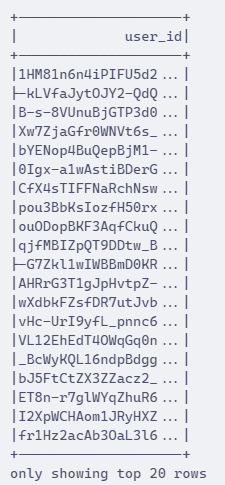
\includegraphics[width=0.3\linewidth]{images/influencers.png}
    \caption{List of influencers}
    \label{fig:influencers}
\end{figure}

The next step was to find the most popular businesses, those that had been left a review by more than 5 influencers. This was done in a very similar way to finding the influencers themselves. First, the number of influencer reviews, that is, reviews from influencers, each business had was calculated. First the reviews were filtered by those that had been reviewed by an influencer. This was done using an inner join between the DataFrame of reviews, and that of the influencers. Since an inner join leaves out rows that do not contain a match in either DataFrame, only the reviews authored by influencers remained. 

\begin{minted}{python}
influencerReviews = reviews.join(influencers, "user_id", "inner")
\end{minted}

Next, the same procedure as above was used to count the numbers of reviews for each business. Since reviews were now filtered by those left by influencers, this effectively counted the number of influencer reviews left at each business, again using the \texttt{groupBy} and \texttt{agg} methods from PySpark, as well as the counting trick.

\begin{minted}{python}
influencerReviewCount = influencerReviews.groupBy("business_id").agg(
    F.count(F.lit(1)).alias("num_influencer_reviews")
)
\end{minted}

Finally, to find the popular businesses with more than 5 influencer reviews, another trivial filter can be applied.

\begin{minted}{python}
popularBusinesses = influencerReviewCount.filter(
    influencerReviewCount.num_influencer_reviews > 5
)
popularBusinesses.show()
\end{minted}

See Figure \ref{fig:popular_businesses} for a shortlist of popular businesses, the output from the above code.

\begin{figure}
    \centering
    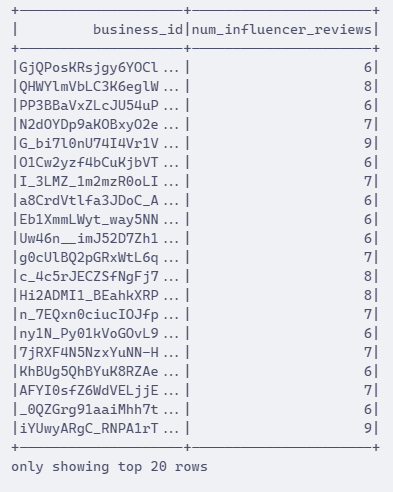
\includegraphics[width=0.5\linewidth]{images/popular_businesses.png}
    \caption{Popular businesses: businesses reviewed by more than 5 influencers.}
    \label{fig:popular_businesses}
\end{figure}

% Question 2
% Did you observe a difference in the amount of authenticity language used in the different
% areas? Explain the steps you took to arrive at the conclusion. Include a screenshot of the
% results (or sample of it). (10%)
\subsection{Analysing authentic language}
I also analysed the reviews for their use of authentic language linked to various cuisines. This involved finding food reviews, determining for each review whether it was authentic, as well as what cuisine was reviewed. I started by determining authenticity. A review was determined authentic if it contained any of the words "authentic", "veritable" or "legitimate". This was done by reducing the DataFrame of reviews by using the PySpark \texttt{where} and \texttt{reduce} methods for filtering, as well as the \texttt{lower} and \texttt{like} functions for the filter condition.

\begin{minted}{python}
authent_words = ["authentic", "veritable", "legitimate"]
authentic_reviews = reviews.where(
    reduce(
        lambda a, b: a|b,
        (lower(reviews.text).like(f'%{word}%') for word in authent_words)
    )
)
num_authentic = authentic_reviews.rdd.count()
num_total = reviews.rdd.count()
print(num_authentic)
# 129945
\end{minted}

This simply checked for each review whether it contained any of the words deemed to be indicators of authenticity, and removed those that did not. The next step was to determine which cuisine the reviews referring to. This was done by looking at the review categories. Each Yelp review contains a list of categories the review belongs to. These categories refer to establishments such as "Casino" and "Hotel", but also restaurants and their cuisines, such as "Sri Lankan" and "Indian". To assign a cuisine to each review, I therefore manually investigated the review categories to determine the major unique Yelp cuisines, then compiled a list of these.
\begin{minted}{python}
cuisines = [
    "Indian",         "Taiwanese",      "Chinese",        "American (Traditional)",
    "American (New)", "French",         "Mexican",        "Vietnamese",
    "Lebanese",       "Greek",          "Italian",        "Trinidadian",
    "Filipino",       "Cuban",          "Korean",         "Thai",
    "Japanese",       "Hawaiian",       "Latin American", "Peruvian",
    "Spanish",        "Ukrainian",      "Irish",          "Brazilian",
    "Senegalese",     "Argentine",      "German",         "Sri Lankan",
    "Soul Food",      "Ethiopian",      "Caribbean",      "Mediterranean",
    "African",        "Middle Eastern"
]
\end{minted}
I then used PySparks \texttt{udf} or User Defined Function feature to create a function that assigns a given review a specific cuisine if it contains one of the above cuisines, or \texttt{None} if none were found. The function was then applied to the DataFrame of reviews and businesses, where its result was added as a new column:
\begin{minted}{python}
def find_cuisine(categories):
    for cuisine in cuisines:
        if cuisine in categories:
            return cuisine
    return None
find_cuisine_udf = udf(find_cuisine, StringType())

reviews_business = reviews.join(business, on="business_id")
reviews_business_cuisines = reviews_business.withColumn(
    "cuisine", find_cuisine_udf(reviews_business.categories)
)
\end{minted}
To ensure only reviews of food were included, I also added a filter that removed any reviews that did not include the "food" category:
\begin{minted}{python}
reviews_business_cuisines_food = reviews_business_cuisines.filter(
    lower(reviews_business_cuisines.categories).contains('food')
)
\end{minted}

To determine the prevalence of authentic language for each cuisine, I filtered the food reviews by those that contained authentic languages by using the aforementioned technique to only include reviews that mentioned authentic words. By then grouping by cuisine and counting the number of reviews for each cuisine, I finally arrived at a DataFrame that showed a breakdown over the number of authentic reviews for each cuisine, shown in figure \ref{fig:auth_cuisines}

\begin{minted}{python}
authentic_reviews_business_cuisines_food = reviews_business_cuisines_food.where(
    reduce(
        lambda a, b: a|b,
        (lower(reviews_business_cuisines_food.text)\
            .like('%' + word + '%') for word in authent_words)
    )
)
authentic_reviews_count_by_cuisine = authentic_reviews_business_cuisines_food\
    .groupBy("cuisine").agg(
        F.count(F.lit(1)).alias("num_reviews_authentic")
    ).sort("cuisine")
authentic_reviews_count_by_cuisine\
    .sort("num_reviews_authentic", ascending=False)\
    .show(authentic_reviews_count_by_cuisine.rdd.count())
\end{minted}

\begin{figure}
    \centering
    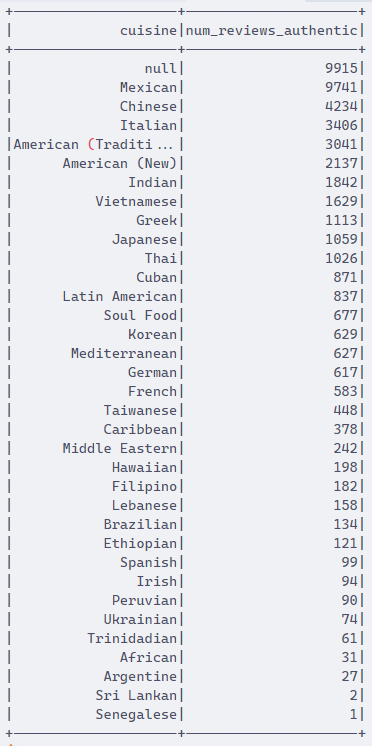
\includegraphics[width=0.5\linewidth]{images/num_auth_cuisines.png}
    \caption{Number of authentic reviews for each cuisine}
    \label{fig:auth_cuisines}
\end{figure}

This by itself did not give much information, as any notable difference in the number of authentic reviews may simply be a result of that cuisine having more overall reviews. I therefore calculated the percentage of reviews for each cuisine that contained authentic language, by counting the number of reviews within each cuisine, and then dividing the number of authentic reviews by the total number of reviews for each cuisine. 

\begin{minted}{python}
reviews_count_by_cuisine = reviews_business_cuisines_food\
    .groupBy("cuisine").agg(
        F.count(F.lit(1)).alias("num_reviews_all")
    ).sort("cuisine")
reviews_counts_percentages = authentic_reviews_count_by_cuisine\
    .join(reviews_count_by_cuisine, "cuisine")\
    .withColumn(
        "reviews_percent_authentic",
        (F.col("num_reviews_authentic") / F.col("num_reviews_all"))
    )
display = reviews_counts_percentages\
    .select("cuisine", "num_reviews_all", "reviews_percent_authentic")\
    .withColumn("reviews_percent_authentic", (F.col("reviews_percent_authentic") * 100))\
    .sort("reviews_percent_authentic", ascending=False)
display.show(display.rdd.count())
\end{minted}

The results of this is shown in Figure \ref{fig:auth_cuisines_percent}.

\begin{figure}
    \centering
    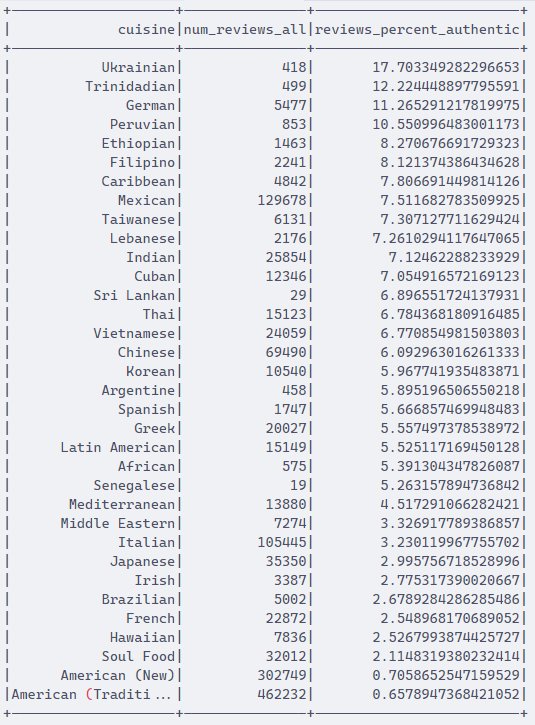
\includegraphics[width=0.5\linewidth]{images/auth_reviews_percent.png}
    \caption{Percentage of reviews that include authentic language for each cuisine}
    \label{fig:auth_cuisines_percent}
\end{figure}

From Figure \ref{fig:auth_cuisines_percent} we can see that a significantly higher percentage of Yelp reviews use authentic language to describe Ukranian cuisine when compared to, say, American cuisine. American cuisine may be so low on the list as a majority of Yelp users are likely American, and thus don't consider their own cuisine authentic.
Based on the number of reviews however, it may be hard to conclude that the percentages displayed in Figure \ref{fig:auth_cuisines_percent} are general tendencies. As an example, Ukranian cuisine only has 418 reviews, and so the high percentage of authentic reviews may be a result of either random noise in the sample, or due to a cultural under-representation of Ukranian food.

\subsection{Authenticity, negativity and stereotypes}

The hypothesis with this data was that reviews that contained both negatibe and authentic language tended to be about non-"western" restaurants (western here referring mainly to the anglicized parts of the world with), such as Asian and Mexican cuisines. To explore this, I wanted to see what percentage of reviews for each cuisine were both authentic and negative, as well as compare this percentage across wester/european vs. non-wester/european cuisines.

I did this by first defining a review as negative or positive if it included negative or positive words respectively. See the code below for a list of positive and negative words. This resultet in 2 DataFrames: one for authentic and positive reviews, as well as one for authentic and negative reviews:

\begin{minted}{python}
neg_words  = [ "dirt",      "kitsch",    "cheap",      "rude",
              "simple",     "bland",     "dodgy",      "poison" ]
pos_words  = [ "clean",     "refined",   "elegant",    "stylish" ]
auth_words = [ "authentic", "veritable", "legitimate" ]

rest_rs = business[
    business.categories.contains('Restaurants')
].join(reviews, "business_id")
rest_rs = rest_rs.withColumn("isAuthentic", rest_rs.text.rlike(f'({")|(".join(auth_words)})'))
rest_rs = rest_rs.withColumn("isNeg", rest_rs.text.rlike(f'({")|(".join(neg_words)})'))
rest_rs = rest_rs.withColumn("isPos", rest_rs.text.rlike(f'({")|(".join(pos_words)})'))
rest_rs = rest_rs.withColumn("cuisine", find_cuisine_udf(rest_rs.categories))
rrs_auth = rest_rs.where(rest_rs.isAuthentic)
rrs_auth_neg = rrs_auth.where(rrs_auth.isNeg)
rrs_auth_pos = rrs_auth.where(rrs_auth.isPos)
\end{minted}

Like earlier, I could then count the number of negative and positive reviews for each cuisine using the PySpark \texttt{groupBy} and \texttt{agg} methods. This gave me a DataFrame where each row is a cuisine, and column for negative and positive review counts. To this I also added the total number of reviews, as well as calculating the fraction of negative and positive reviews for each cuisine based on these figures.

\begin{minted}{python}
neg_cuis = rrs_auth_neg.groupBy("cuisine").agg(
    F.count(F.lit(1)).alias("neg")
)
pos_cuis = rrs_auth_pos.groupBy("cuisine").agg(
    F.count(F.lit(1)).alias("pos")
)
cuis_revs = neg_cuis.join(pos_cuis, on="cuisine")
reviews_count_by_cuisine = rest_rs.groupBy("cuisine").agg(
    F.count(F.lit(1)).alias("tot_revs")
)
cuis_revs = cuis_revs.join(reviews_count_by_cuisine, "cuisine")

cuis_revs = cuis_revs.withColumn("neg_p", (cuis_revs.neg / cuis_revs.tot_revs) * 100)
cuis_revs = cuis_revs.withColumn("pos_p", (cuis_revs.pos / cuis_revs.tot_revs) * 100)

cuis_revs.show(cuis_revs.rdd.count())
\end{minted}

\begin{figure}
    \centering
    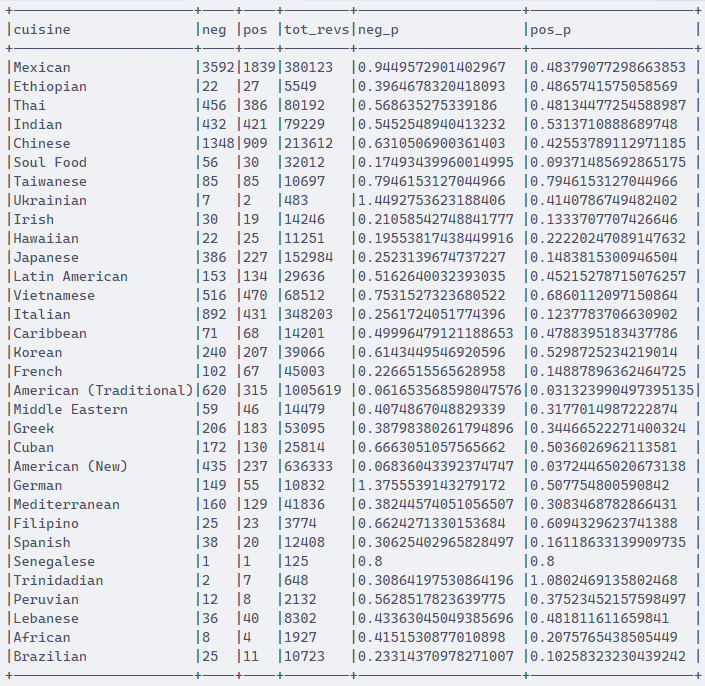
\includegraphics[width=0.5\linewidth]{images/negposcount.png}
    \caption{Negative, positive and total review count by cuisine.}
    \label{fig:negposcount}
\end{figure}

See Figure \ref{fig:negposcount} to see the DataFrame generated by the above code. It is important to again mention that these counts are of reviews that are both considered authentic as well as positive/negative. In actuality, there are significantly more positive/negative reviews, but most of them do not contain authentic language. The fractions in the DataFrame have also been multiplied by 100 for readability. Already we can see that, for example, the Mexican cuisine has more negative than positive reviews, having around 0.9\% negative reviews and 0.5\% positive.

From this table, I calculated the average negative and positive fraction of reviews for cuisines determined to be western and non-western. A western cuisine was determined to be cuisines often associated with high-end dining experiences. See the below code for a list of western cuisines. This resulted in a final DataFrame that included figures for average fraction of positive reviews and the average fraction of negative reviews for both western and non-western cuisines.

\begin{minted}{python}
western_cuisines = [
    "American (New)", "American (Traditional)", "French", "German",   "Greek",
    "Hawaiian",       "Mediterranean",          "Italian" "Japanese", "Irish"
]

cuis_revs = cuis_revs.withColumn("isWestern", cuis_revs.cuisine.isin(western_cuisines))

ctr_p = cuis_revs.groupBy("isWestern").agg(F.mean("pos_p"), F.mean("neg_p"))
ctr_p.show(ctr_p.rdd.count(), False)
\end{minted}

\begin{figure}
    \centering
    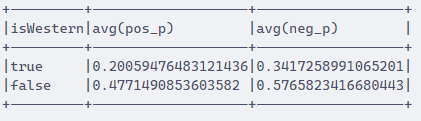
\includegraphics[width=0.5\linewidth]{images/finalpscores.png}
    \caption{Table of average positive review percentage and negative review percentage for both western and non-western cuisines.}
    \label{fig:finalpscores}
\end{figure} 

The DataFrame from the above is displayed in Figure \ref{fig:finalpscores}. As we can see from the table, there is a higher fraction of negative reviews for both western and non-western cuisines, though western cuisine has around 0.14\% more negative than positive reviews, where non-western cuisines only have around 0.1\%. The most notable difference between western and non-western cuisines is that botn the positive and the negative fraction is significantly higher for non-western cuisines. This is likely fraction of "authentic" reviews being higher for non-western cuisines, thus inflating the overall number of reviews captured.

While the results don't show anything that would confirm that negative authentic language is more prevalent for non-western cuisines, it does show that non-western cuisines tend to be described by authentic language more often than western cuisine. As mentioned earlier, this may be due to the demographic of the review website Yelp being predominantly westerners that do not consider their own cuisine "authentic".

\subsection{Machine learning on Spark}

Finally, I trained a linear regression model on various features of the reviews to predict the number of stars a review would give. First, I used the existing binary features included in the data. This was whether a review was cool, funny, and useful. Then, I included the number of reviews held by the particular business being reviewed. I then engineered features based on authenticity, negative and positive language by counting the number of authentic, negative and positive words used in the review respectively. The next feature I created was based on the review date. Both year, month and day of the review were used as three separate features. Finally, I also used the American state that the business was located in by one-hot encoding it into 27 different binary variables. In total, I had the following features:

\begin{minted}{python}
features = [
    "cool",  "funny", "useful",     "review_count", "year",
    "month", "day",   "auth_count", "neg_count",    "pos_count",
] + states # list of US states
\end{minted}

I trained a Linear Regression model to predict the review star count. This was done using Cross-Validation, by randomly splitting the reviews into 5 splits. Then training on 4 of the splits, and evaluating on the 5th. This was repeated until all 5 splits had been evaluated once, and the evaluation metrics were averaged. Using Cross Validation ensures that the result is representative of what you can expect to see when evaluating on unseen data.

The optimization metric I chose was Sum of Squared Error (SSE). SSE is the most common metric used when training Linear Regression models. The squared error is calculated by taking the square of the difference between the prediction and the true value:
$$
\text{squared error}=\left(Y_i-\hat{Y}_i\right)^2
$$
The square is used both to ensure that the error is always positive, as well as to punish large errors exponentially more than small errors. The sum of all these errors is then taken to be the models current performance:
$$
\text{SSE}=\sum_{i=1}^N \left(Y_i-\hat{Y}_i\right)^2
$$
The goal of the model is to minimize this value by finding the line of best fit, which can be done analytically.

For evaluating the final results of the model, I used both Mean Squared Error (MSE) and Adjusted $R^2$. MSE is similar to SSE, but takes the mean instead of the sum of the squared errors. This is helpful to see if there are some very large errors in the final model, as the SSE would change significantly based on the number of predictions. Adjusted $R^2$ is a variant of the popular $R^2$ metric. $R^2$ is a metric that measures how well the linear regression model fits the data, or more specifically, it measures the proportion of the total variation in the dependent variable that is explained by the predictor variables. $R^2$ is a very popular metric to use, but it has some shortcomings, especially when using Multiple Linear Regression. $R^2$ fails to take into account the number of predictors in the model, and will always prioritise models with more predictors. Since I made use of quite a lot of predictors, I used Adjusted $R^2$ in hopes of comparing different nested models with each other, though I did not end up implementing this. Despite this, Adjusted $R^2$ is still a useful metric to determine how well the model fits the data.

The result of training the model using 5 folds of cross-validation and averaging the results are given in Table \ref{table:mlresults}

\begin{table}[]
    \centering
    \begin{tabular}{|l|l|l|}
        \hline
                                 & MSE & Adj. $R^2$ \\ \hline
5-split Cross Validation results & 1.98 & 0.0939 \\ \hline
    \end{tabular}
    \caption{Results from training a Linear Regression model through 5-fold cross validation.}
    \label{table:mlresults}
\end{table}

The results aren't great, with an Adjusted $R^2$ of only 0.09. This indicates that most of the variance isn't explained by the predictors, and thus, the model is not very good at predicting the number of stars a review will give. Improvements could probably be made by doing regularization and removing unneeded features, doing more data preprocessing such as LDA or PCA, and even using a language model to make predictions based on the entire review text.